\documentclass[11pt,fleqn]{exam}
\usepackage[utf8]{inputenc}

\usepackage[margin=1in]{geometry}
\usepackage{amsmath,amssymb}
\usepackage{wasysym}
\usepackage{gensymb}
\usepackage{multicol}
\usepackage{float}
\usepackage{graphicx}
\usepackage{units,icomma}

\usepackage{xcolor}
\usepackage[colorlinks,linkcolor=blue,urlcolor=blue]{hyperref}
\usepackage[margin=1.5cm]{caption}

%\usepackage{lipsum}
%\usepackage[printwatermark]{xwatermark}
%\newwatermark[allpages,color=blue!7,angle=45,scale=2,xpos=0,ypos=0]{ridlow.wordpress.com}

\hyphenation{
  chro-no-ampe-ro-met-ric
  ber-dia-me-ter
  de-ngan
  me-nem-pati
  mic-ro-graphs
  di-ban-ding}

\renewcommand{\figurename}{Gambar.}
\def\equationautorefname{Persamaan}
\newcommand{\class}{OLIMPIADE ASTRONOMI}
\newcommand{\term}{Tingkat Kabupaten/Kota - 2019}
\newcommand{\examnum}{OSK Astronomi 2019}
%\newcommand{\examdate}{11/02/2014}
%\newcommand{\timelimit}{120 Minutes}

\pagestyle{head}
\firstpageheader{}{}{}
\runningheader{\examnum}{}{Halaman \thepage\ dari \numpages}
\runningheadrule


\begin{document}

\noindent
\begin{tabular*}{\textwidth}{l @{\extracolsep{\fill}} r @{\extracolsep{6pt}} l}
\textbf{\class}  \\ %& \textbf{Name:} & \makebox[2in]{\hrulefill}\\
\textbf{\term}  %&&\\
%\textbf{\examnum} &&\\
%\textbf{\examdate} &&\\
%\textbf{Time Limit: \timelimit} & Teaching Assistant & \makebox[2in]{\hrulefill}
\end{tabular*}\\
\rule[2ex]{\textwidth}{2pt}

\noindent
\begin{tabular}{ll}
Copyright (c) 2019 & Sulistiyowati (sulis.astro08@gmail.com)\\
                   & Ridlo W. Wibowo (ridlo.w.wibowo@gmail.com)
                   
\end{tabular}

\vspace{0.3cm}
\noindent
Solusi ini dibuat tanpa jaminan kesesuaian dengan solusi resmi dari juri olimpiade sains bidang Astronomi. Pengguna boleh menyebarluaskan dan/atau memodifikasi solusi ini dengan mencantumkan sumber asli. Hak cipta soal ada pada Kemendiknas dan dilindungi undang-undang.

\vspace{0.4cm}
\noindent
\rule[2ex]{\textwidth}{1.5pt}

\textbf{SOAL PILIHAN GANDA}

\begin{questions}

\question Bagi pengamat di dekat ekuator, kedudukan titik Aries tertinggi saat Matahari terbenam akan berlangsung pada
\begin{choices}
\choice 21 Maret
\choice 21 Juni
\choice 22 Desember
\choice 21 Juni
\choice 23 September
\end{choices}

\textit{Jawaban: }C\\
Titik Aries ($\gamma$) atau titik musim semi (\textit{vernal equinox}) adalah salah satu dari dua titik perpotongan antara ekliptika dengan ekuator. Posisi tertinggi titik Aries di langit adalah ketika ia di meredian pengamat $\rightarrow HA_{\gamma}=0^{jam}$; untuk pengamat di ekuator titik Aries saat itu tepat ada di zenith. 

Bagi pengamat di ekuator, Matahari terbenam saat sudut jamnya bernilai sekitar $HA_{\odot}=6^{jam}$.
\begin{eqnarray*}
HA_{\odot}+RA_{\odot} &=& LST = HA_{\gamma},\\
6^{jam}+RA_{\odot}&=&0^{jam},\\
RA_{\odot}&=&-6^{jam}=18^{jam},
\end{eqnarray*}
bersesuaian dengan tanggal 22 Desember.

\question Andaikan orbit Matahari mengelilingi pusat Galaksi Bima Sakti berbentuk lingkaran. Jarak Matahari ke pusat Galaksi adalah $2\times 10^9$ sa. Jika waktu yang diperlukan Matahari untuk satu kali mengelilingi pusat Galaksi adalah 200 juta tahun, serta dengan mengabaikan pengaruh dari materi gelap/\textit{dark matter}, maka massa Galaksi yang terkandung di dalam orbit Matahari yang dinyatakan dalam $M_{\odot}$ adalah
\begin{choices}
\choice $8\times 10^4$
\choice $2\times 10^{10}$
\choice $2\times 10^{11}$
\choice $1\times 10^2$
\choice $10^{10}$
\end{choices}

\textit{Jawaban: }C\\
Untuk \underline{$r$, $P$, dan $M$ secara berturut-turut dalam sa, tahun, dan $M_{\odot}$}, maka berlaku:
\begin{eqnarray*}
M(r)&=&\frac{r^3}{P^2}\\
M(r)&=&\frac{(2\times 10^9)^3}{(200\times 10^6)^2}\\
M(r)&=&2\times 10^{11} M_{\odot},
\end{eqnarray*}
dengan $M(r)$ menyatakan massa yang terlingkupi oleh radius $r$.

\question Sebuah lensa konvergen dengan panjang fokus $f$ untuk membuat bayangan dari sebuah objek yang berjarak 10 m dari lensa. Bayangan yang terbentuk berada pada jarak 10 cm. Berapakah $f$ dalam cm?
\begin{choices}
\choice $9,00$
\choice $9,90$
\choice $10,0$
\choice $10,1$
\choice $11,1$
\end{choices}

\textit{Jawaban: }B\\
Lensa konvergen adalah lensa yang sifatnya mengumpulkan cahaya $\rightarrow$ lensa cembung. Berlaku persamaan:
\begin{eqnarray*}
\frac{1}{f}&=&\frac{1}{s}+\frac{1}{s'}\\
\frac{1}{f}&=&\frac{1}{1000 \text{ cm}}+\frac{1}{10 \text{ cm}}\\
\frac{1}{f}&=&0,101\\
f&=&9,90 \text{ cm}.
\end{eqnarray*}

\question Assuming constant luminosity of the Sun for about 10 billion years since zero age main sequence, the percentage of the solar mass which was converted to energy through fusion reaction in its core during that time is
\begin{choices}
\choice $0,02$ \%
\choice $0,20$ \%
\choice $0,07$ \%
\choice $0,70$ \%
\choice $0,34$ \%
\end{choices}

\textit{Jawaban: }C\\
During that time ($\Delta t$), the energy released by the Sun ($E$) with constant luminosity $L$ which can be taken from the table of constant is:
\begin{eqnarray*}
E&=&L \cdot \Delta t\\
E&=&3,96\times 10^{26} \text{ Watt}\times 10^{10} \text{ years}\times 365,25 \frac{\text{days}}{\text{year}}\times 24 \frac{\text{hours}}{\text{day}}\times 3600 \frac{\text{seconds}}{\text{hour}}\\
E&=&1,25\times 10^{44} \text{ Joule}.
\end{eqnarray*}

This energy is generated from the conversion of $\Delta m$ mass into energy under the equation:
\begin{eqnarray*}
E&=&\Delta m \cdot c^2\\
\Delta m&=&\frac{E}{c^2}\\
\Delta m&=&\frac{1,25\times 10^{44} \text{ Joule}}{(3\times 10^8 \text{ }\frac{\text{m}}{\text{s}})^2}\\
\Delta m&=&1,39\times 10^{27} \text{ kg}.
\end{eqnarray*}
In solar masses percentage:
\begin{eqnarray*}
\frac{\Delta m}{M_{\odot}}&=&\frac{1,39\times 10^{27} \text{ kg}}{1,99\times 10^{30} \text{ kg}}\times 100\%\\
\frac{\Delta m}{M_{\odot}}&=&6,98\times 10^{-4}\times 100\%\\
\frac{\Delta m}{M_{\odot}}&=&0,07\%.
\end{eqnarray*}

\question Nilai $x$ dari persamaan berikut $(a^x)^2 \exp^{\ln a}=1$ adalah
\begin{choices}
\choice 1
\choice -1 atau 1
\choice 0
\choice -1/2
\choice 1/2
\end{choices}

\textit{Jawaban: }D\\
Ingat bahwa $\ln$ adalah logaritma basis $e$, 

$\ln y = ^e\log y=\frac{\log y}{\log e}$.

Mari belajar logaritma; dan logaritma natural ($\ln$)

Cara 1, kedua ruas dilogaritmakan dengan basis 10, menjadi:
\begin{eqnarray*}
\log [(a^x)^2 \exp^{\ln a}]&=&\log 1\\
\log a^{2x}+\log e^{\ln a}&=&0\\
2x\log a+\ln a \log e&=&0\\
2x\log a+ ^e\log a \log e&=&0\\
2x\log a+\frac{\log a}{\log e} \log e&=&0\\
(2x + 1) \log a  &=&0\\
2x+1&=&0\\
x&=&-\frac{1}{2}.
\end{eqnarray*}

Cara 2, kedua ruas dilogaritmakan dengan basis $e$, menjadi:
\begin{eqnarray*}
\ln [(a^x)^2 \exp^{\ln a}]&=&\ln 1\\
\ln a^{2x}+\ln e^{\ln a}&=&0\\
2x\ln a+\ln a \ln e&=&0\\
(2x + 1) \ln a &=&0\\
2x+1&=&0\\
x&=&-\frac{1}{2}.
\end{eqnarray*}

Cara 3,
\begin{eqnarray*}
	(a^x)^2 e^{\ln a}&=& 1\\
	a^{2x} a &=& 1\\
	a^{2x + 1} &=& 1\\
	2x+1&=&0\\
	x&=&-\frac{1}{2}.
\end{eqnarray*}

Catatan: \\
Solusi tunggal di atas hanya berlaku untuk $a \neq 1$. \\
Jika $a = 1$, solusinya banyak: $x = -1/2, 0, 1/2, \sqrt{2}, \pi, \infty, \ldots$ dan lain sebagainya tak hingga banyaknya, karena 1 pangkat berapapun tetap 1. 

\question Terdapat tiga titik P(1,1,1), Q(2,3,4), dan R(5,6,7) yang membentuk sebuah bidang. Jika terdapat titik S(-2,5,10), maka jarak minimum titik S ke bidang PQR adalah
\begin{choices}
\choice $\sqrt{3}$
\choice $6/\sqrt{3}$
\choice $\sqrt{6}/4$
\choice $\sqrt{6}/3$
\choice $6/\sqrt{3}$
\end{choices}

\textit{Jawaban: } D\\
Cara 1:\\
Jarak terpendek titik S ke bidang PQR bisa dicari dengan menghitung besar vektor yang tegak lurus bidang dan vektor itu harus melalui titik S, misal sebut saja vektor $\overrightarrow{\text {ST}}$ digambarkan di bawah ini berwarna biru (lihat gambar bagian kiri terlebih dahulu).
\begin{figure}[h!]
\centering
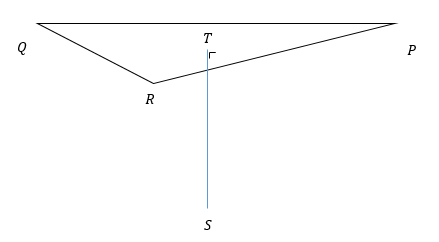
\includegraphics[scale=0.65]{pqr1.PNG}
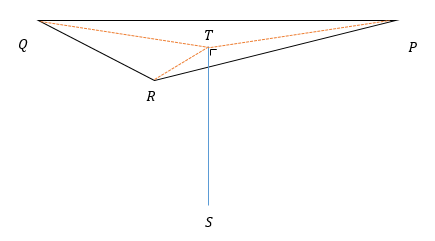
\includegraphics[scale=0.65]{pqr2.PNG}
\caption*{Catatan: Dalam gambar-gambar di sini, vektor hanya digambarkan sebagai garis saja, meskipun cara paling tepat untuk menggambarkan vektor adalah dengan menggunakan anak panah.}
\end{figure}
Vektor $\overrightarrow{\text {ST}}$ harus tegak lurus terhadap vektor-vektor yang digambarkan berwarna oranye (lihat gambar bagian kanan). Artinya, hasil perkalian titik (\textit{dot product}) vektor-vektor berwarna oranye terhadap vektor berwarna biru harus sama dengan nol. Anggap T($a,b,c$), maka:\\
\begin{eqnarray*}
\overrightarrow{\text {ST}}\cdot \overrightarrow{\text {PT}}&=&0\\
(a+2)(a-1)+(b-5)(b-1)+(c-10)(c-1)&=&0\\
a^2+a+b^2-6b+c^2-11c&=&-13\hspace{1cm}(1)\\
\overrightarrow{\text {ST}}\cdot \overrightarrow{\text {QT}}&=&0\\
(a+2)(a-2)+(b-5)(b-6)+(c-10)(c-7)&=&0\\
a^2+b^2-8b+c^2-14c&=&-51\hspace{1cm}(2)\\
\overrightarrow{\text {ST}}\cdot \overrightarrow{\text {RT}}&=&0\\
(a+2)(a-5)+(b-5)(b-6)+(c-10)((c-7)&=&0\\
a^2-3a+b^2-11b+c^2-17c&=&-90\hspace{1cm}(3)\\
\end{eqnarray*}
Eliminasi secara berturut-turut
\begin{itemize}
\item persamaan (1) dan (2), diperoleh \hspace{1cm}$a+2b+3c=38\hspace{1cm}(4)$
%\item persamaan (1) dan (3), diperoleh \hspace{0.8cm}$4a+5b+6c=77\hspace{1cm}(5)$
\item persamaan (2) dan (3), diperoleh \hspace{1.4cm}$a+b+c=13\hspace{1cm}(5)$
\item persamaan (4) dan (5), diperoleh \hspace{1.9cm}$b+2c=25\hspace{1cm}(6)$
\end{itemize}
Kemudian substitusikan nilai $b$ dari persamaan (6) ke persamaan (5):
\begin{eqnarray*}
a+b+c&=&13\\
a+25-2c+c&=&13\\
a&=&c-12
\end{eqnarray*}
Gunakan nilai $a$ dan $b$ sebagai fungsi $c$ tersebut untuk dimasukkan ke persamaan (2), boleh juga yang lain, maka:
\begin{eqnarray*}
a^2+b^2-8b+c^2-14c&=&-51\hspace{1cm}(2)\\
(c-12)^2+(25-2c)^2-8(25-2c)+c^2-14c&=&-51\\
6c^2-122c+620&=&0\\
3c^2-61c+310&=&0
\end{eqnarray*}
Cari $c$ sebagai akar persamaan kuadrat tersebut.
\begin{eqnarray*}
c_{1,2}&=&\frac{61\pm\sqrt{(-61)^2-4(3)(310)}}{2(3)},
\end{eqnarray*}
didapat:\\
$c_1=\frac{31}{3}, b_1=13/3, a_1=-5/3$ sehingga T\textsubscript{1}($\frac{-5}{3},\frac{13}{3},\frac{31}{3}$)\\
atau\\
$c_2=10, b_2=5, a_2=-2$ sehingga T\textsubscript{2}($-2, 5, 10$) $\rightarrow$ sama dengan S, sehingga nilai ini tidak mungkin dipilih.\\
Jadi, titik T harus sama dengan T\textsubscript{1}. Jarak terpendek $=|\overrightarrow{\text{ST}}|$.
\begin{eqnarray*}
|\overrightarrow{\text{ST}}|&=&\sqrt{(\frac{-5}{3}+2)^2+(\frac{13}{3}-5)^2+(\frac{31}{3}-10)^2}\\
&=&\sqrt{\frac{6}{9}}\\
&=&\frac{\sqrt{6}}{3}.
\end{eqnarray*}

Cara 2:\\
Cari hasil operasi perkalian silang (\textit{cross product}) antara dua vektor yang berada di bidang PQR untuk memperoleh vektor normal bidang (vektor yang tegak lurus terhadap arah bidang). 
\begin{eqnarray*}
\overrightarrow{\text{N}}&=&\overrightarrow{\text{PR}}\times\overrightarrow{\text{PQ}}\\
&=&((5-1)\hat{i}+(6-1)\hat{j}+(7-1)\hat{k})\times((2-1)\hat{i}+(3-1)\hat{j}+(4-1)\hat{k})\\
&=&(4\hat{i}+5\hat{j}+6\hat{k})\times(\hat{i}+2\hat{j}+3\hat{k})\\
&=&-3\hat{i}+6\hat{j}-3\hat{k}
\end{eqnarray*}

Buatlah vektor yang melalui salah satu dari ketiga titik pembentuk bidang (misal dipilih titik P) dan titik S, $\overrightarrow{\text{PS}}=(-2-1,5-1,10-1)=(-3,4,9)$. Jarak terpendek $r$ dari titik S ke bidang adalah $|\overrightarrow{\text{PS}}|\cos \theta$, dengan $\theta$ menyatakan sudut antara vektor normal $\overrightarrow{\text{N}}$ dengan vektor $\overrightarrow{\text{PS}}$. Lihat gambar berikut.
\begin{figure}[h!]
\centering
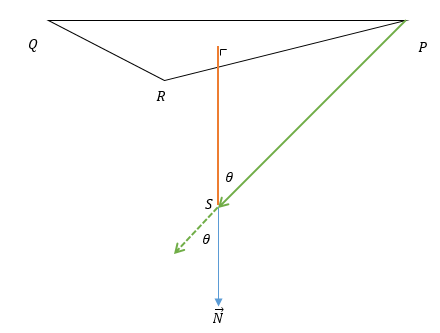
\includegraphics[scale=0.8]{pqrcross.PNG}
\caption*{Garis oranye tebal menunjukkan panjang $r$ yang menyatakan proyeksi vektor $\overrightarrow{\text{PS}}$ ke vektor normal $\overrightarrow{\text{N}}$.}
\end{figure}

Gunakan \textit{dot product}.
\begin{eqnarray*}
\overrightarrow{\text{N}}\cdot\overrightarrow{\text{PS}} &=& |\overrightarrow{\text{N}}||\overrightarrow{\text{PS}}|\cos \theta\\
r = |\overrightarrow{\text{PS}}|\cos\theta &=& \frac{\overrightarrow{\text{N}}\cdot\overrightarrow{\text{PS}}}{|\overrightarrow{\text{N}}|} \qquad = \overrightarrow{\text{PS}} \cdot \hat{n} \\
&=&\frac{(-3,6,-3)\cdot(-3,4,9)}{\sqrt{(-3)^2+6^2+(-3)^2}}\\
&=&\frac{6}{\sqrt{54}}\\
&=&\frac{6}{\sqrt{6}\sqrt{9}}\\
&=&\frac{\sqrt{6}}{3}.
\end{eqnarray*}

\question Terdapat dua vektor gaya $\overrightarrow{F}_{1} = 10(\hat{i}, 2\hat{j}, 3\hat{k})$ N dan $\overrightarrow{F}_{2} = 5(\hat{i}, 3\hat{j}, 5\hat{k})$ N yang bekerja pada suatu benda. Hal ini mengakibatkan benda berpindah dengan vektor perpindahan $\overrightarrow{r} = (10\hat{i}, 10\hat{j}, 5\hat{k})$ m. Usaha yang dilakukan gaya tersebut, dalam satuan Nm, adalah
\begin{choices}
\choice 150
\choice 225
\choice 300
\choice 775
\choice 900
\end{choices}

\textit{Jawaban: } D\\
Resultan gaya $\Sigma\overrightarrow{F}=\overrightarrow{F}_1+\overrightarrow{F}_2=15\hat{i}+35\hat{j}+55\hat{k}$.\\
Usaha/kerja $W=\Sigma\overrightarrow{F}\cdot\overrightarrow{r}=(15, 35, 55)\cdot(10, 10, 5)= 150 + 350 + 275 = 775$ Joule.

\question Jika atom hidrogen yang berada di tingkat energi dasar ditembak dengan seberkas partikel, maka akan terjadi eksitasi ke level energi yang lebih tinggi karena proses tumbukan tersebut. Berapakah energi kinetik minimum yang harus dimiliki partikel tersebut untuk terjadinya eksitasi ini dan sesuai dengan garis apakah energi foton tersebut?
\begin{choices}
	\choice $2,18 \times 10^{-18}$ J dan Balmer Alfa
	\choice 13,6 eV dan H$\alpha$ 
	\choice $1,63 \times 10^{-18}$ J dan Lyman Alfa
	\choice 13,6 eV dan Lyman Alfa
	\choice 10,2 eV dan H$\alpha$
\end{choices}

\textit{Jawaban: } C\\
Energi minimum mengindikasikan transisi (dalam hal ini eksitasi) yang terjadi adalah ke kulit terdekat setelah tingkat energi dasar yakni ke $n=2$.
\begin{eqnarray*}
E_{min}&=&E_{n=2}-E_{n=1}\\
&=&-\frac{13,6 \text{ eV}}{2^2}-\left(-\frac{13,6 \text{ eV}}{1^2}\right)\\
&=&10,2\text{ eV}\\
&=&1,63\times 10^{-18}\text{ Joule}.
\end{eqnarray*}

Transisi antara $n=1$ ke $n=2$ atau sebaliknya masuk kategori garis Lyman Alfa, besar panjang gelombangnya:
\begin{eqnarray*}
E &=&\frac{hc}{\lambda}\\
1,63\times 10^{-18}\text{ Joule}&=&\frac{6,63\times 10^{-34}\text{ J s}\times 3\times 10^8\text{ m/s}}{\lambda}\\
\lambda&=&1218,75\text{ \AA} \qquad (UV).
\end{eqnarray*}

\question Andaikan kamu berada di Merkurius yang berjarak 0,39 sa ke Matahari. Pilihlah pernyataan yang benar mengenai kecerlangan Matahari.
\begin{choices}
\choice Fluks Matahari di Bumi lebih lemah 1,64 kali daripada di Merkurius
\choice Fluks Matahari di Merkurius lebih terang 6,57 kali daripada di Bumi
\choice Fluks Matahari di Merkurius lebih terang 2,56 kali daripada di Bumi
\choice Fluks Matahari di Bumi lebih lemah 0,61 kali daripada di Merkurius
\choice Fluks Matahari di Merkurius lebih terang 0,39 kali daripada di Bumi
\end{choices}

\textit{Jawaban: } B\\
Perbandingan fluks 
$$\frac{F_M}{F_\oplus}= \left(\frac{d_\oplus}{d_M}\right)^2= \left(\frac{1}{0,39}\right)^2=6,575$$ 

atau $F_\oplus / F_M = 0,1521$.

\question Dalam fotometri fotoelektrik Bintang Pollux, laju cacah yang diukur pada tanggal 15:00 UT adalah 175000 cacah per detik dan 350000 cacah per detik pada pukul 16:00 UT. Laju cacah pada pada pukul 15:45 UT berdasarkan interpolasi linier adalah 
\begin{choices}
\choice 291250 cacah per detik
\choice 301250 cacah per detik
\choice 361250 cacah per detik
\choice 381250 cacah per detik
\choice 391250 cacah per detik
\end{choices}

\textit{Jawaban: } tidak ada pilihan yang benar\\
Untuk interpolasi linier, nilai suatu titik di antara dua titik didekati dengan garis lurus.
\begin{eqnarray*}
n_1&=&mt_1+c\\
350.000&=&m(16)+c\hspace{1cm}(1)\\
n_2&=&mt_2+c\\
175.000&=&m(15)+c\hspace{1cm}(2)
\end{eqnarray*}
Eliminasi persamaan (1) dan (2) sehingga diperoleh $m=175.000$ cacah per detik per jam dan $c=-2.450.000$ cacah per detik. Maka untuk $t_3$=15:45 UT = 15,75\\ $n_3=175.000(15,75)-2.450.000=306.250$ cacah per detik.

\question Sudut kritis pada Hukum Snellius terjadi jika sudut bias membentuk sudut sebesar 90 derajat. Seberkas sinar merambat dari medium rapat ke medium renggang. Jika indeks bias air sebesar 1,33 dan indeks bias \textit{crown glass} sebesar 1,52, maka sudut kritisnya adalah sebesar
\begin{choices}
\choice 41,1\degree
\choice 48,6\degree
\choice 50,0\degree 
\choice 61,0\degree 
\choice 63,1\degree 
\end{choices}

\textit{Jawaban: } D\\
\begin{eqnarray*}
n_1\sin \theta_1&=&n_2\sin \theta_2\\
1,52\sin \theta_1&=&1,33\sin 90\degree\\
\sin \theta_1&=&0,875\\
\theta_1&=&61,04\degree.
\end{eqnarray*}

\question Kecepatan orbit suatu satelit di orbit rendah Bumi (\textit{Low Earth Orbit}, LEO), dengan ketinggian sekitar 200 km dari permukaan Bumi, adalah
\begin{choices}
\choice 1,022 km s$^{-1}$
\choice 2,4 km s$^{-1}$
\choice 4,63 km s$^{-1}$
\choice 7,8 km s$^{-1}$
\choice 29,8 km s$^{-1}$
\end{choices}

\textit{Jawaban: } D\\
\begin{eqnarray*}
v&=&\sqrt{\frac{GM_{\oplus}}{R_{\oplus}+h}}\\
&=&\sqrt{\frac{6,67\times 10^{-11}\times 5,97\times 10^{24}}{(6378\text{ km}+200\text{ km})\times 10^3}}\\
&=&7,78\times 10^3 \quad \text{m/s}\\
&=&7,8 \quad \text{km/s}.
\end{eqnarray*}

\vspace{0.5cm}
\textbf{Pilihan Ganda Kompleks}

\textbf{Pilihlah}
\begin{choices}
\choice \textbf{jika 1, 2, dan 3 benar}
\choice \textbf{jika 1 dan 3 benar}
\choice \textbf{jika 2 dan 4 benar}
\choice \textbf{jika 4 saja benar}
\choice \textbf{jika semua benar}
\end{choices}

\question Diketahui spektrum dari objek-objek astronomi sebagai berikut. Pilihlah pernyataan yang benar.

\begin{figure}[ht!]
\centering
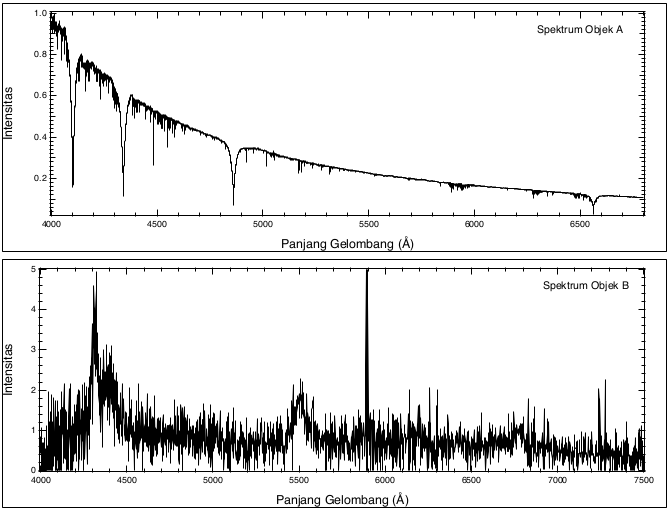
\includegraphics[scale=0.55]{spektrum.png}
\end{figure}
\begin{enumerate}
	\item Spektrum objek B merupakan spektrum galaksi
	\item Spektrum objek A merupakan spektrum bintang kelas G
	\item Spektrum objek A merupakan spektrum bintang kelas A
	\item Spektrum objek B merupakan spektrum \textit{planetary nebulae}
\end{enumerate}

\textit{Jawaban: } B\\
Spektrum objek A menunjukkan profil mendekati satu benda hitam berpuncak pada panjang gelombang yang lebih pendek dari 4000 dengan garis-garis absorpsi $\rightarrow$ paling mirip dengan spektrum bintang kelas A.

Spektrum objek B menunjukkan profil kombinasi banyak benda hitam dengan banyak absorpsi dan garis emisi $\rightarrow$ paling mirip dengan spektrum galaksi.

Maka, pernyataan 1 dan 3 saja yang benar.

\question Tanggal 1 Januari 2010 M bertepatan dengan persitiwa bulan purnama (fase Bulan hari ke-14 atau ke-15). Peristiwa yang bertepatan seperti itu terjadi setiap 235 kali periode sinodis Bulan. Peristiwa yang mirip dengan tahun baru 2010 M tersebut terjadi juga pada
\begin{enumerate}
\item 1 Januari 1991 M
\item 1 Agustus 2029 M
\item 1 Januari 2029 M
\item 1 Juni 1990 M
\end{enumerate}

\textit{Jawaban: } B\\
Total jumlah hari untuk 235 kali periode sinodis Bulan:\\
$$N=235\times 29,530589\text{ hari}=6.939,69\text{ hari}$$
$$N=\frac{6.939,69\text{ hari}}{365,25\frac{\text{ hari}}{\text{ tahun}}}\simeq19\text{ tahun}.$$

Di antara pilihan 1 hingga 4, yang memiliki selisih 19 tahun dengan 1 Januari 2010 M adalah 1 Januari 1991 dan 1 Januari 2029.

Maka pernyataan 1 dan 3 saja yang benar. 

\question Berikut ini merupakan citra Matahari yang diamati pada tanggal 13 November 2015 dengan filter H$\alpha$. Pilihlah pernyataan yang benar.
\begin{figure}[h!]
\centering
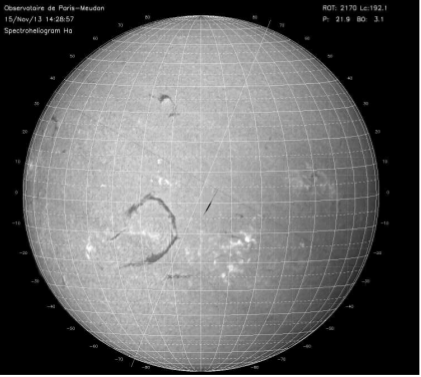
\includegraphics[scale=0.7]{matahari.png}
\end{figure}
\begin{enumerate}
\item Terdapat lebih dari tiga bintik Matahari pada citra.
\item Terdapat filamen Matahari pada citra.
\item Terdapat hubungan antara Bintik Matahari dengan medan magnet Matahari.
\item Terdapat Korona Matahari pada citra.
\end{enumerate}

\textit{Jawaban: } A\\
Daerah dengan banyak aktivitas magnetik (bintik Matahari) pada citra yang diambil menggunakan filter H$\alpha$ tampak sebagai daerah atau titik-titik putih. Dalam citra yang ditunjukkan pada soal, di area separuh piringan ke bawah banyak terdapat fitur ini, mengindikasikan banyaknya bintik Matahari. Filamen terlihat jelas sebagai fitur garis melengkung di piringan Matahari. Korona merupakan fitur dengan temperatur sangat tinggi yang tidak bisa diamati menggunakan filter H$\alpha$.\\
Maka, pernyataan 1, 2, dan 3 saja yang benar.

%\vspace{0.5cm}
\newpage
\textbf{ESSAY SINGKAT}

\question Sisa supernova berekspansi ke segala arah dengan laju 1000 km per detik. Jika sisa supernova ini berjarak 10000 parsek dari Bumi, berapakah perubahan diameter sudut setelah setahun? Apakah perubahan ini dapat diamati dengan teleskop landas Bumi berdiameter 3,8 meter? (Dalam hal ini, turbulensi atmosfer tidak dapat diabaikan)

\textit{Jawaban:}\\
Selama $\Delta t=1\text{ tahun}$, perubahan radius:
\begin{eqnarray*}
\Delta r&=&v\Delta r\\
&=&1000\text{ }\frac{\text{km}}{\text{s}}\times 1\text{ th}\times 365,25\text{ }\frac{\text{hari}}{\text{th}}\times 24\text{ }\frac{\text{jam}}{\text{hari}}\times 3600\text{ }\frac{\text{s}}{\text{jam}}\\
&=&3,155\times 10^{10}\text{ km}.
\end{eqnarray*}
Perubahan diameter: $\Delta D=2\Delta r=6,31\times 10^{10}\text{ km}$.
Perubahan diameter sudut:
\begin{eqnarray*}
\Delta\delta&=& 2 \arctan (\frac{\Delta r}{d\text{ (jarak)}})\\
&=&2 \arctan(\frac{3,155\times 10^{10}\text{ km}}{10^4\text{ pc}\times 206.265\text{ }\frac{\text{ sa}}{\text{ pc}}\times 1,496\times 10^8\text{ }\frac{\text{km}}{\text{sa}}})\\
&=&1,17\times 10^{-5}\text{ derajat}\\
&=&0,0422''.
\end{eqnarray*}

Resolusi teoretik untuk teleskop optik ($\lambda_\text{observasi}=5.500\AA$):\\
\begin{eqnarray*}
\theta&=&\frac{1,22\lambda}{D_\text{teleskop}}\\
&=&\frac{1,22\times 5.500\text{\AA}\times 10^{-10}\text{ }\frac{\text{m}}{\text{\AA}}}{3,8\text{ m}}\\
&=&1,77\times 10^{-7}\text{ radian}\\
&=&0,0364''.
\end{eqnarray*}
Dengan tidak mengabaikan turbulensi atmosfer, meskipun resolusi teoretik teleskop lebih baik dibanding ukuran benda yang ingin tampak dipisahkan, ukuran dalam orde seperseratus detik busur tidak bisa dipisahkan karena adanya \textit{seeing}. Seeing terbaik di permukaan Bumi ${\sim}0,4$ detik busur. Untuk mengatasi masalah ini, teleskop optik landas Bumi berdiameter besar menerapkan teknologi \textit{adaptive optic} jika ingin mendapat citra dengan resolusi tinggi.


\question Jika kita menganggap Jupiter sebagai benda hitam yang memancarkan energi sebesar yang diterima dari Matahari, tentukan berapakah temperatur permukaan Jupiter? Pada kenyataannya, Jupiter memiliki temperatur sebesar 145$^{\circ}$C. Hitung rasio antara temperatur Jupiter sebagai benda hitam dengan temperatur Jupiter sebenarnya. Jelaskan secara singkat sumber panas Jupiter!

\textit{Jawaban:} \\
Jupiter sebagai benda hitam:
\begin{eqnarray*}
\text{Daya diserap}&=&\text{Daya dipancarkan}\\
\text{Fluks Matahari di Jupiter} \times \pi R_J^2&=&4\pi R_J^2\sigma T_J^4\\
\frac{L_{\odot}}{4\pi d_J^2}&=&4\sigma T_J^4\\
T_J&=& \left(\frac{L_{\odot}}{16\pi d_J^2\sigma} \right)^{\frac{1}{4}}\\
&=& \left(\frac{3,96\times 10^{26}\text{ Watt}}{16\pi(7,7833\times 10^{11}\text{ m})^2\times 5,67\times 10^{-8}\text{ }\frac{\text{Watt}}{\text{m}^2\text{ K}^4}} \right)^{\frac{1}{4}}\\
&=&123,063\text{ K} \quad \text{atau} \quad -150^{\circ}\text{C}.
\end{eqnarray*}
Temperatur Jupiter teramati: $145\degree\text{C}+273=418$ K. Rasio: $\frac{123,063}{418}=0,29$.\\
Panas Jupiter kemungkinan bersumber dari energi dalammya yang berasal dari keruntuhan gravitasi pada awal masa pembentukannya.

\question Festival Tanabata merupakan perayaan yang berkaitan dengan musim panas yang dirayakan di beberapa negara seperti Jepang, Cina, Mongolia, dan Korea. Legenda Tanabata mengisahkan Bintang Vega dan Bintang Altair yang dipisahkan Sungai Amanogawa (Galaksi Bima Sakti). Diketahui koordinat ($\alpha$, $\delta$) Vega dan Altair masing-masing adalah (18$^\text{j}$36$^\text{m}$56$^\text{d}$, 38$^{\circ}$47'01'') dan (19$^\text{j}$50$^\text{m}$47$^\text{d}$, 08$^{\circ}$52'06''). Tentukan jarak sudut antara Vega dan Altair (dalam derajat).

\textit{Jawaban: }\\
Sketsa:
\begin{figure}[h!]
\centering
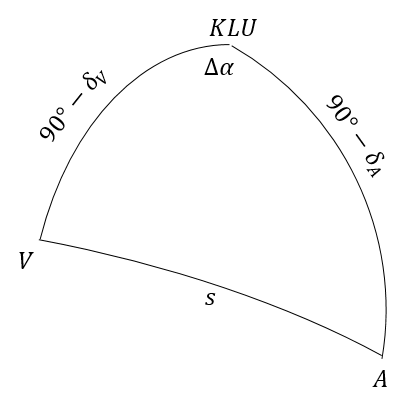
\includegraphics[scale=0.8]{segbol.PNG}
\end{figure}

\begin{eqnarray*}
\delta_V&=& \left(38+\frac{47}{60}+\frac{1}{3600}\right)\degree =38,78361\degree \\
\delta_A&=& \left(8+\frac{52}{60}+\frac{6}{3600}\right)\degree =8,8683\degree \\
\Delta\alpha&=&\alpha_V-\alpha_A=1^\text{j}13^\text{m}51^\text{d}=\left(1+\frac{13}{60}+\frac{51}{3600}\right)^{\text{jam}}\times 15\degree{/\text{jam}}=18,4625\degree
\end{eqnarray*}
Jarak antara Vega dan Altair di langit $s$:
\begin{eqnarray*}
\cos s&=&\cos(90\degree-\delta_V)\cos(90\degree-\delta_A)+\sin(90\degree-\delta_V)\sin(90\degree-\delta_A)\cos \Delta\alpha\\
&=&\sin \delta_V\sin \delta_A+\cos \delta_V\cos \delta_A\cos \Delta\alpha\\
&=&0,827\\
s&=&34,1957\degree\\
&=&34\degree11'44''69 \simeq 34\degree.
\end{eqnarray*}


\question Dua orang astronom, yang terpisah oleh jarak 100 km pada garis utara\--selatan, secara simultan mengamati sebuah asteroid di dekat zenith. Hasil pengamatan mereka menunjukkan bahwa paralaks asteroid tersebut sebesar 5 detik busur. Hitunglah jarak ke asteroid (dalam satuan km). Berapakah perbandingan jarak asteroid tersebut dengan jarak ke Bulan?

\textit{Jawaban: }\\
Dengan asumsi asteroid ada di bagian tengah langit antara dua pengamat, dapat disketsakan:
\begin{figure}[h!]
\centering
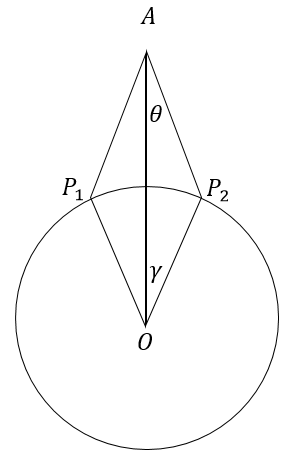
\includegraphics[scale=0.8]{asteroid.PNG}
\end{figure}

Sudut $\theta=$ paralaks asteroid $=5''$. 

Sudut $\gamma$ bisa dicari dengan
\begin{eqnarray*}
\frac{\gamma}{360\degree} &=& \frac{\frac{1}{2}\times\text{jarak pengamat}}{\text{keliling Bumi}}\\
\frac{\gamma}{360\degree} &=& \frac{50\text{ km}}{2\pi(6378\text{ km})}\\
\gamma &\simeq& 0,449167\degree	
\end{eqnarray*}

Dengan aturan sinus dan $OA=d_A$ menyatakan jarak asteroid:
\begin{eqnarray*}
\frac{\sin \theta}{R_{\oplus}}&=&\frac{\sin(180\degree-\gamma-\theta)}{d_A}\\
d_A&=&\frac{\sin(180\degree-\gamma-\theta)}{\sin \theta}R_{\oplus}\\
&=&324,397R_{\oplus}\\
&=&2.069.004\text{ km}\\
\end{eqnarray*}
Perbandingan jarak ke asteroid terhadap jarak ke Bulan:
\begin{equation}
\frac{d_{A}}{d_{\leftmoon}} = \frac{2.069.004\text{ km}}{384.400\text{ km}} = 5,3824 \simeq 5,38
\end{equation}

Catatan:\\
Karena jarak pengamat $P_1$ dan $P_2$ tidak terlalu besar, asumsi Bumi datar masih bisa digunakan, menghasilkan nilai yang serupa; $d_A = 2062650 + 6378$ km, $\frac{d_{A}}{d_{\leftmoon}}$ = 5,3825.


\question Sebuah bintang serupa Matahari (massa dan radius sama dengan yang dimiliki Matahari) dianggap mengubah seluruh energi potensial gravitasi yang dimilikinya menjadi pancaran energi radiasi sehingga luminositas sebesar $L_{\odot}$ dihasilkan hingga kematiannya. Hitunglah nilai perkiraan energi potensial gravitasi bintang, lalu hitunglah umur bintang jika anggapan ini digunakan.

\textit{Jawaban: }\\
\begin{eqnarray*}
E_\text{pot. grav}&=&\frac{GM^2}{R}\\
&=&\frac{6,67\times 10^{-11}(1,99\times 10^{30})^2}{6,96\times 10^8}\\
&=&3,795\times 10^{41}\text{ Joule}.\\
\Delta t&=&\frac{E_\text{pot. grav}}{L_{\odot}}\\
&=&\frac{3,795\times 10^{41}}{3,96\times 10^{26}}\\
&=&9,58\times 10^{14}\text{ detik}\\
&=&3,04\times 10^7\text{ tahun}.
\end{eqnarray*}

Catatan:\\
Energi potensial bola gas dengan kerapatan konstan dapat dihitung dengan integral menghasilkan\\
$E_\text{pot. grav} = \frac{3 G M^2}{5 R}$


\end{questions}


\vspace{2cm}
\begin{flushright}
Solusi seperti ini dapat diperoleh di \url{http://ridlow.wordpress.com}
\end{flushright}
\end{document}
